\subsubsection{} Генерация криптографических ключей.
\label{sec:eng:performance:rsakeygen}

Метод \texttt{generateRSAKeyPair} необходим для генерации пары \textit{RSA} ключей (публичного и приватного), а метод \texttt{generateAESKey} -- для генераци симметричного \textit{AES} ключа. В листинге \ref{sec:eng:performance:rsakeygen:code} приведён код для тестирования метода генерации пары \textit{RSA} ключей, а на рисунках \ref{sec:eng:performance:rsakeygen:result} и \ref{sec:eng:performance:aeskeygen:result} результаты измерений генерации \textit{RSA} и \textit{AES} ключей соответственно.

\begin{code}
  \lstinputlisting{inc/src/perf/rsakeygen.swift}
   \caption{Тестовый метод для метода генерации пары RSA ключей}
   \label{sec:eng:performance:rsakeygen:code}
\end{code}

\begin{figure}[h]
\centering
\begin{minipage}{.5\textwidth}
  \centering
  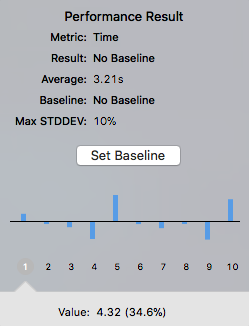
\includegraphics[width=.65\linewidth]{inc/img/perf/rsakeygen.png}
  \captionof{figure}{Результаты замеров генерации RSA ключа}
  \label{sec:eng:performance:rsakeygen:result}
\end{minipage}%
\begin{minipage}{.5\textwidth}
  \centering
  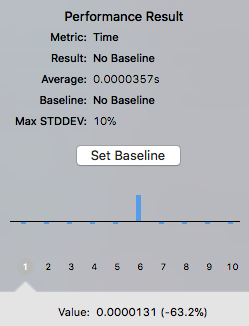
\includegraphics[width=.65\linewidth]{inc/img/perf/aeskeygen.png}
  \captionof{figure}{Результаты замеров генерации AES ключа}
  \label{sec:eng:performance:aeskeygen:result}
\end{minipage}
\end{figure}

\FPEval{\rsaKeyGenMesaureMax}{62.4}
\FPEval{\rsaKeyGenMesaureMin}{11.3}
\FPEval{\rsaKeyGenMesaureAverage}{32.1}
\FPEval{\perfDevRSAKeyGen}{\rsaKeyGenerationMaxValue - (\rsaKeyGenMesaureMax + \rsaKeyGenMesaureMin + \rsaKeyGenMesaureMin) \ 3}

Рассчитаем отклонение от предельно допустимого значения генерации \textit{RSA} ключа, подставив значения в формулу (\ref{perfDifEquation}):
\begin{center}
\(\perfDev = \num{\rsaKeyGenerationMaxValue} - \frac{\num{\rsaKeyGenMesaureMax} + \num{\rsaKeyGenMesaureMin} + \num{\rsaKeyGenMesaureAverage}}{3} = \num{perfDevRSAKeyGen} \, сек\)
\end{center}